\chapter{Theoretical background}
In this chapter the different terminologies used in this report will be introduced and the importance in context to this research will be discussed. 

\section{Energy management in buildings}
\begin{wrapfigure}{o}{0.5\textwidth}
    \centering
    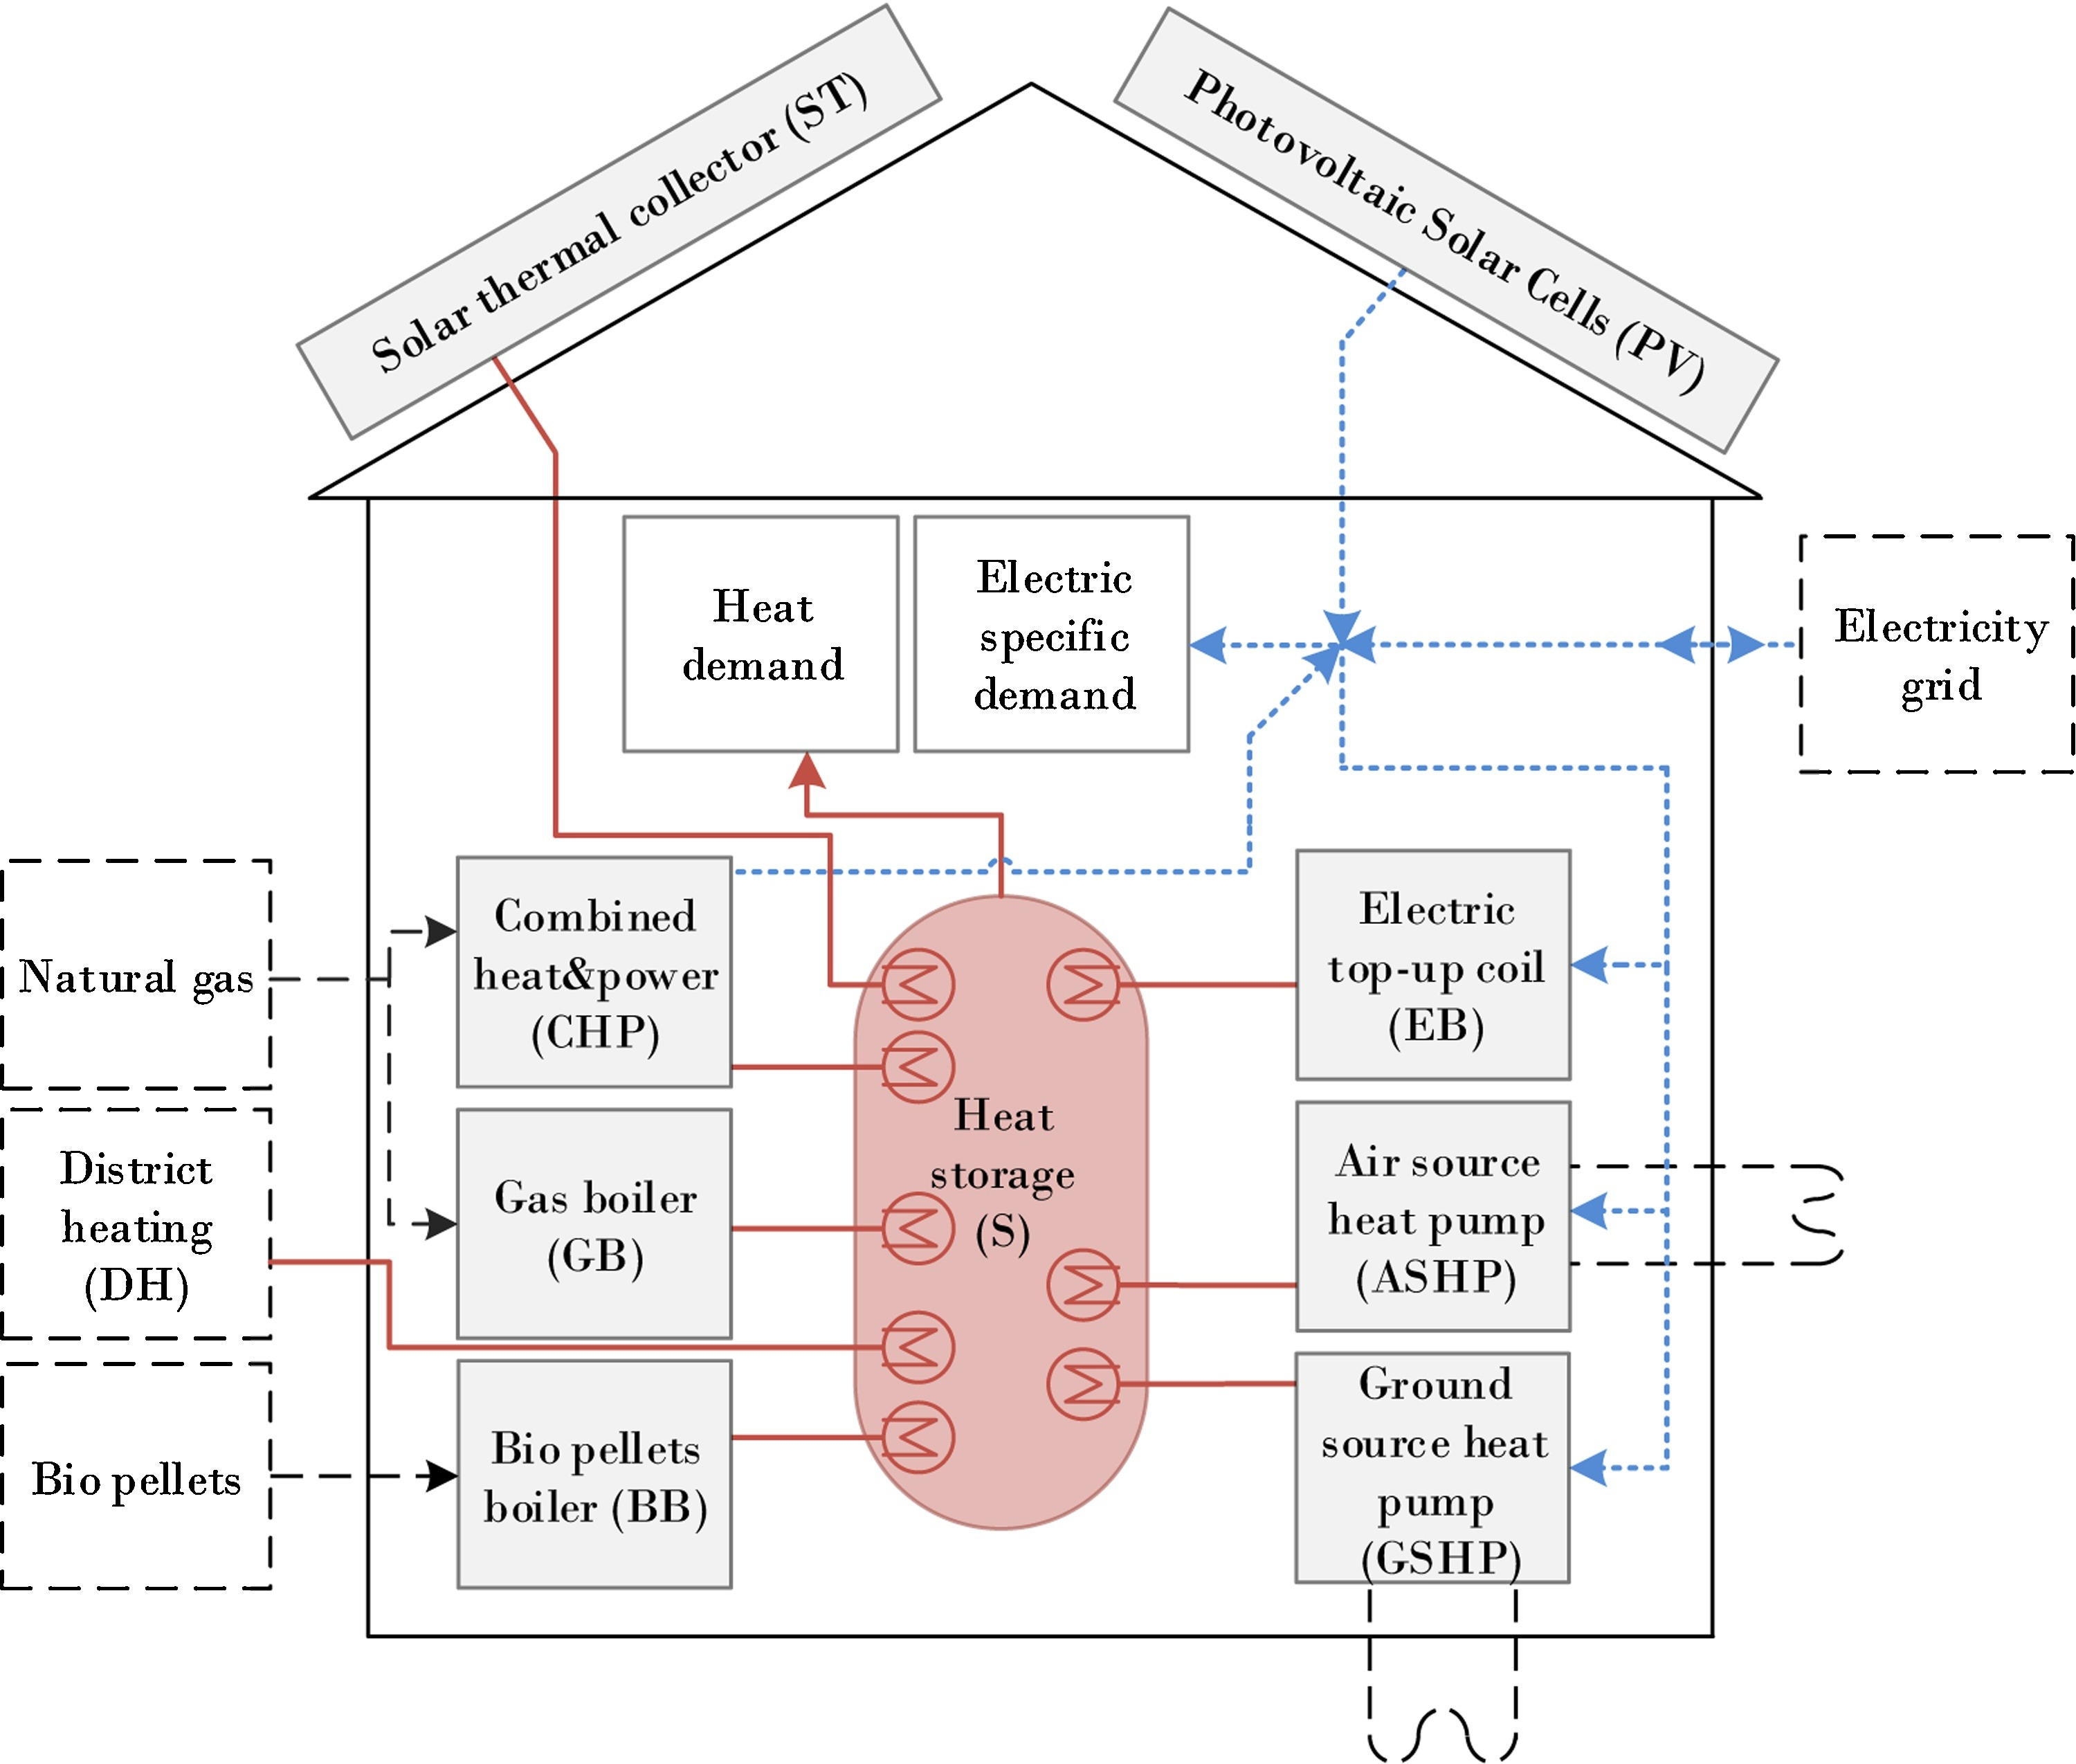
\includegraphics[width=0.45\textwidth]{vedlegg/grid.jpg}
    \caption{\textit{An example of a building, including building installations with connection to electricity grid}}
    \label{fig:gridl}
\end{wrapfigure}

A building is defined as a permanent or temporary structure enclosed by a building envelope, including building installations. The main purpose for a building is to give protection against external climate and disturbances. The buildings also need to provide a healthy and comfortable indoor environment without causing unreasonable high expenses in regards of investment and operational costs of the building. Net Zero Energy Buildings (\ac{nzeb}s) are buildings that aim to minimize the environmental impact by reducing the energy demand and producing on site renewable energy that compensates for the energy demand. The term net is used to refer to that the building is connected to the energy infrastructure and underlines the fact that there is a balance between energy taken from and supplied back to the energy grid over a period of time. An illustration of a building including an example of building installations is displayed in figure \ref{fig:gridl}.

The energy consumption of a building is affected by the external climate, the building envelope, technical installations, operation and maintenance. The operation and maintenance is depending on the occupant behaviour and wanted indoor environmental conditions and are referred to as human influenced factors. External climate, the building envelope and building installations are, unlike the human influenced factors, factors that can not be controlled. 
\pagebreak

\begin{wrapfigure}{i}{0.5\textwidth}
    \centering
   %\vspace{1mm}
    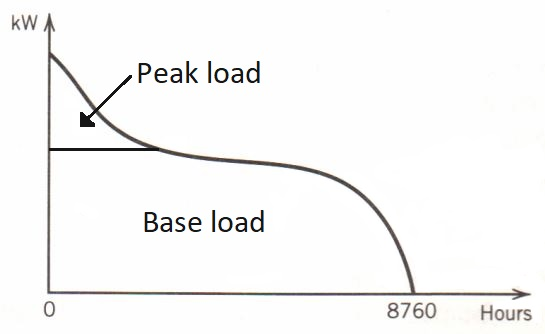
\includegraphics[width=0.5\textwidth]{vedlegg/loaddur}
    \caption{Load duration curve over a year}
    %\vspace{18mm}
    \label{fig:ldc}
\end{wrapfigure}

The energy consumption of a building is defined by the energy need for space heating and cooling, ventilation, domestic hot water, lighting and equipment. Internal- and solar gains are also taken into account when calculating energy demand. To design the optimal solution for each building, a load duration curve should be used to ensure correct sizing of the HVAC components. A load duration curve, illustrated in figure \ref{fig:ldc}, is an estimation of total energy demand over a year and describes the size and duration of different heat or cooling demands. A system with low operation cost should be installed to cover the base load which could cover between 90-95\% of total energy demand. The reason its not desirable to cover the entire energy demand is the high investment cost for the effect needed, so a system with a low investment cost should therefore be installed to cover the peak load, even though it has a higher operation cost. 
%An air tight envelope with low heat transfer coefficient (U-value) in the building materials ensures a low energy demanding building.

\section{Heat transfer}
\begin{wrapfigure}{0}{0.5\textwidth}
    \centering
   \vspace{5mm}
    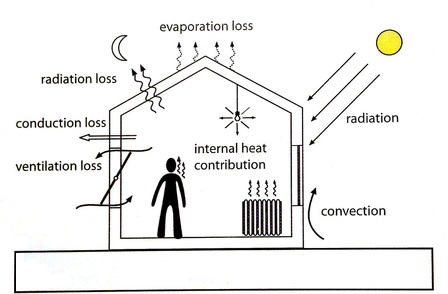
\includegraphics[width=0.5\textwidth]{vedlegg/7281185.jpg}
    \caption{Heat balance in a building \cite{dahl}.}
    \label{fig:ccr}
\end{wrapfigure}

Heat is transferred through either conduction, convection, radiation or evaporation. In practice in a building it is a combination of conduction, convection and radiation. 

The heat balance of the building is illustrated in figure \ref{fig:ccr} with the different parameters that has an influence on the heat transfer. It is the thermal transmittance of the building envelope, also known as U-value, that decides how much heat that is transferred through the building. The better a building is insulated, the lower the U-value is and less heat is transferred through the envelope. To calculate the U-value, the thermal resistance, R, needs to be calculated in each layer. The R-value through construction materials is found by dividing the thickness (t) by the thermal conductivity ($\lambda$) of the material as shown in equation \ref{eq:R}. 

\begin{equation}
    R = \frac{t}{\lambda} \hspace{5mm} [K m^2/W]
    \label{eq:R}
\end{equation}

The U-value is calculated using equation \ref{eq:U}.

\begin{equation}
    \label{eq:U}
    U = \frac{1}{\sum R} \hspace{5mm} [W/m^2 K]
\end{equation}

The U-value alone does not describe all of the heat loss because thermal bridges appear typically in connection points between constructions. This is parts where the thermal resistance is significantly lower than rest of the construction and the heat loss is higher. This needs to be taken into account, and prevented as much as possible. 

\begin{equation}
    Q = U \cdot A \cdot \Delta T [W]
\end{equation}

\section{Indoor Environment and Thermal Comfort}
A study done in 2001 showed that people spent in average almost 87\% of their life inside buildings, either at home or at work \cite{Nhaps}. It is therefore obvious that the indoor environment has an enormous impact on human health and well being. Productivity is related to the ability to perform various tasks and studies have shown a clear connection between productivity and indoor environment. The noise level, temperature and perceived air quality are all parameters that has an effect on the productivity level. Studies have shown that people perform tasks more accurately, faster and over a longer time with increased productivity. Other consequences are that people feel healthier, sustain stress more effectively and enjoy spending time at work. Less sick leave and improved performance is very economically beneficial for a company.
Indoor environment can be defined as a composite of the five elements; Thermal-, atmospheric-, acoustic-, actinic-, and mechanical environment. The acoustic and mechanical environment has no impact on the energy use or operation costs and will not be discussed further in this report.

The thermal environment depends on the indoor air temperature, surface temperatures, temperature gradients, relative humidity and air velocity. The thermal comfort is defined as 'that condition of mind which expresses satisfaction with the thermal environment' (NS-EN ISO 7730), and depends also on the clothing level and activity level. Clothing level describes the thermal resistance between the surface of the skin and the outer surface of the clothing, with the unit clo. Activity level is a measure of the metabolic rate from energy production by the human body with the unit met. Clothing level is assumed to be equal to 1 clo in the winter and 0.5 clo in the summer. Sedentary activities like office work is equal to 1.2 met. 

$$ 1.0 \hspace{1mm} \mbox{clo} = 0.155 \hspace{1mm} m^2K/W$$
$$ 1.0 \hspace{1mm} \mbox{met} = 58 \hspace{1mm} W/m^2 $$

\begin{wrapfigure}{0}{0.45\textwidth}
    \centering
    \vspace{-4mm}
    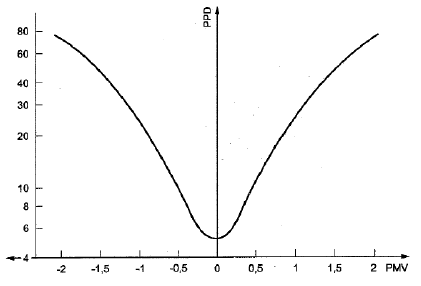
\includegraphics[width=0.4\textwidth]{vedlegg/pmvppd.png}
    \caption{Relation between PMV and PPD}
    \label{fig:my_label}
 \end{wrapfigure}
 
Thermal comfort is an individual perception and it is therefore difficult to make everyone in a room completely satisfied. Predicted Mean Vote (\ac{pmv}) is a psycophysic 7-point scale from -3, cold, to +3, hot where 0 corresponds to thermal neutral, that can be calculated for a given situation. Predicted Percentage of Dissatisfied (\ac{PPD}) can be derived from PMV and is the predicted percent of dissatisfied people at each PMV. The aim is to reach category A, a PPD of 6\% or less. 
%\pagebreak

Figure \ref{fig:opt} shows the optimum operative temperature in category A for different activity and clothing levels. Clothing level 1 clo and activity level 1.2 met gives and optimum operative temperature of 21.5$^o$C $\pm$ 1$^o$C. Operative temperature (\ac{To}) is defined as "the uniform temperature of an imaginary black enclosure in which an occupant would exchange the same amount of heat by radiation and convection as in the actual non-uniform environment(ISO 7730:2005). With metabolic rates between 1.0 and 1.3 and air velocities below 0.10 m/s, operative temperature can be calculated using equation \ref{eq:to}. 

\begin{figure}[h!]
    \centering
    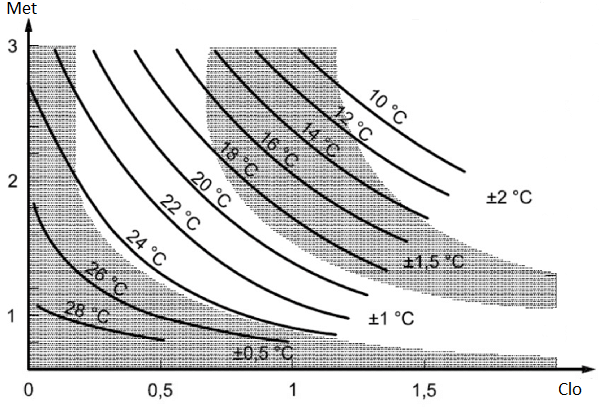
\includegraphics[scale=0.6]{vedlegg/opt.png}
    \caption{Optimum operative temperature category A.}
    \label{fig:opt}
\end{figure}

\begin{equation}\label{eq:to}
    t_o = \frac{(t_a+t_{mr})}{2}
\end{equation}

where,

$t_a$ \hspace{1mm} = Air temperature [$^o$C] \\
$t_{mr}$ = Mean radiant temperature [$^o$C] \\




\begin{table}[h!]
    \centering
        \caption{Design criteria for office building, activity level: 1.2 met, Clothing level: 0.5 clo summer, 1.0 clo winter, category A (ISO 7730).}
        \arrayrulecolor{white}
    \begin{tabular}{p{3.5cm}|p{1.8cm}|p{1.8cm}}
    \rowcolor{denim} \color{white} Parameter & & \\
    \hline
       \rowcolor{lblue} & Summer & Winter  \\
         \hline
         \rowcolor{denim} Operative temp [$^o$C] & 24.5 $\pm$ 1.0 & 22.0 $\pm$ 1.0  \\
    \hline
       \rowcolor{lblue} Relative humidity [\%] & 60 & 40  \\
         \hline
         & &  \\
    \end{tabular}
    \label{tab:design}
    \arrayrulecolor{black}
\end{table}

Atmospheric environment indicates the perceived indoor air quality and depends on the concentration of air pollutants in the indoor air, amount of particles and smell. Ventilation is used to provide good indoor air quality by supplying fresh air and extracting contaminated air. The ventilation rate should be based on pollution load from occupants and materials. Concentration of CO$_2$ is a common way to control the quality of the air. The gas is not toxic for humans at low levels but gives a good indication of how good the air change in a room is. 

Actinic environment is an indication of the quality of light inside the building and is described by the daylight factor. The daylight factor represent the amount of illumination available indoors relative to the illumination present outdoors at the same time under overcast skies.

To obtain good indoor climate, a heating, cooling and ventilation system might be required to be installed, depending on the location and use of the building.



\section{Building Installations}
Building installations include all attached and fixed installations connected to a building. That includes systems for heating, cooling, ventilation and sanitary, which has the collective term HVAC systems. It is also consisting of all electrical and gas installations, fire alarms and fire extinguishing installations and access and intruder control. This research will focus on the systems for space heating and cooling, heating of domestic hot water, photovoltaic panels for electricity production, ventilation system and lighting as they are most relevant for an energy analysis.

\subsection*{Space Heating and Cooling}
A heating system for space heating and heating of domestic hot water will be installed to provide the desired temperatures. A heat pump will be installed to cover the base load for heating. The same heat pump will be used to cover the cooling load. 

\subsection*{Heat Pump}
A Heat Pump (\ac{hp}) is a system that reduces the primary energy use by utilizing renewable energy and can be used for heating and cooling purposes. There exists many different types of heat pumps, with different working fluids, but they are all based on the same main function. The heat pump consists of four main components including a compressor, a condenser, an expansion valve and an evaporator. The evaporator extracts heat from a heat source and transfer the heat to a working fluid. The working fluid transfers thermal energy to the supply system by changing state throughout a continuous cycle driven by the compressor. A simple sketch is shown in figure \ref{fig:HP} to illustrate the principle behind the heat pump.

\begin{figure}[h!]
    \centering
    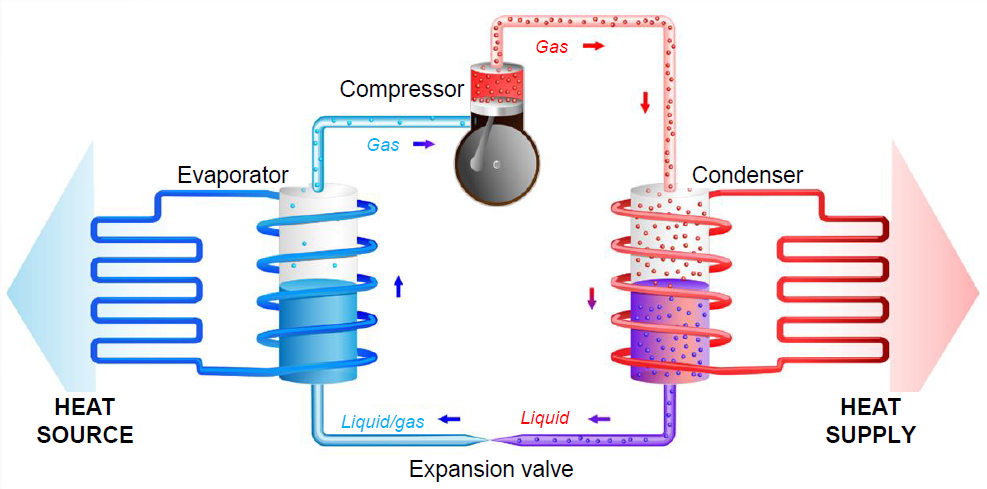
\includegraphics[scale=0.35]{vedlegg/HP.png}
    \caption{Heat pump cycle}
    \label{fig:HP}
\end{figure}

A heat pump has typically a coefficient of performance (\ac{COP}) of between 2 and 5, depending on the type, which means it can reduce the energy demand for space heating and cooling by between 50-80\%. The energy saving can be calculated by using equation \ref{eq:ES}.

\begin{equation}
    \mbox{Energy saved} = 1 - \frac{1}{COP} [\%]
    \label{eq:ES}
\end{equation}

The \ac{COP} can be calculated using equation \ref{eqn:COP} where Q is the delivered heat, and W the necessary work done by the compressor. A heat pump that can deliver a big amount of heat is however often expensive to install so it is therefore beneficial to use to cover the base load for heating and cooling. Primary energy use when using a heat pump can be calculated using equation \ref{eqn:PEU}.

\begin{equation} \label{eqn:COP}
    \mbox{COP} = \frac{\ac{Q}}{\ac{W}}
\end{equation}

\begin{equation}\label{eqn:PEU}
    \mbox{Primary energy use} = \mbox{energy coverage} \cdot \frac{\mbox{Heat demand}}{COP}
\end{equation}

\begin{wrapfigure}{0}{0.35\textwidth}
    \centering
    %\vspace{-4mm}
    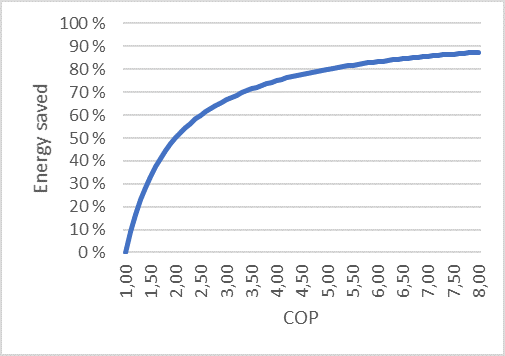
\includegraphics[width=0.35\textwidth]{vedlegg/cop1.png}
    \caption{Relationship between COP and energy savings}
    \label{fig:c}
 \end{wrapfigure}
 
Heat pumps can utilize different types of renewable energy depending on the location and availability of resources. Different sources are ground, ground water, sea water, gray water, sewage and air. Air source is the only source that are available everywhere, and is the one that will be used and discussed in this report. 

\subsubsection*{Air Source Heat Pump (\ac{ASHP})}
Ambient air is the most available heat source for use in a heat pump, has the lowest installation costs and are for those reasons among the most commonly used in heat pumps. A similar heat source is exhaust air from the ventilation system, which has a slightly higher investment cost, but a lower operation cost and maintenance need. Exhaust air also has a more steady, reliable temperature than ambient air. The exhaust air is believed to be the optimal solution for heat source. A air to water heat pump will be used.

\subsection*{Heating system}
Water born heating system

\section{Solar Energy}
For the building to qualify as a \ac{nzeb} it needs to produce on site renewable energy equal to, or greater than, the primary energy use. Solar energy is an important source of renewable energy, and has a potential greater than the total world energy demand. It is however demanding to utilize more than a fraction of that incoming energy. Solar energy can be utilized in the shape of thermal energy by direct solar gains, or by solar thermal collectors. Solar energy can also be converted into electricity by photovoltaics (\ac{pv}), or applied directly as daylight. Solar energy is utilized by transforming solar radiation into heat and electricity and consists of a transformer unit, a distribution system and an energy storage unit. How much energy it is possible to extract depends on solar irradiation and angle of the panels

\subsection{Photovoltaics}
Electricity is generated from solar energy by transforming radiation into electricity using photovoltaic cells before storing the generated power in batteries. The electricity produced can be used directly on site or exported and sold back to the grid depending on the need. \ac{pv} panels produces and stores direct current (DC) electricity which needs to converted by an inverter to an alternating current (AC) used on the grid. Modules commercially available today has an efficiency in the range 15\% to 20\% of irradiation, and can be installed on the outside of the building envelope. This report will investigate how many modules that will be needed to cover the entire demand and what the cost will be. 

\subsection{Solar thermal collector}
Solar thermal collectors are used for space heating or heating of hot water and the efficiency is in the range 40-70\% of irradiation. 

\section{Ventilation system}
The purpose of a ventilation system is to provide good indoor air quality by removing pollutants and odors. This can be achieved by natural forces like wind and pressure difference or by mechanical forces. It is also possible to combine the two methods. The use of natural forces are the most economical in terms of installation cost and operational costs but is very limited in controlling the indoor environment. An office has a high demand for good air quality for good productivity and reducing the risks of sickness. To obtain desired indoor environment a mechanical ventilation system is therefore preferred.

The most common mechanical ventilation methods are mixed and displacement ventilation. Mixed ventilation is based on the principle that all air inside a room is completely mixed with a uniform temperature and pollutant concentration. Fresh air is supplied into the room at high velocities to make that happen. In displacement ventilation utilizes buoyancy forces as colder air is supplied close to the floor before heated up by pollutant sources, rising, bringing contaminants away from the occupied zone before exiting the room close to the ceiling. Displacement ventilation is preferable to use in large rooms with high heat loads. One disadvantage of displacement ventilation is the risk of draft from supplying cold air into the occupied zone. Mixed ventilation is believed to be a better option for the office building

The ventilated air can be supplied and extracted at a constant air volume (\ac{CAV}) or with a variable air volume (\ac{VAV}) with the use of demand controlled ventilation (\ac{DCV}). DCV can use temperature, occupancy or CO$_2$ concentration sensors to decide how much fresh air the ventilation system should provide to maintain good indoor air quality. DCV is a more complex system that has a higher investment cost, but can be cheaper and more accurate in operation. CAV is not as flexible as DCV but also has the possibility of supplying air at different rates according to predefined schedules. The weekly schedule is predefined for the office building.

The chosen ventilation system for the building is mechanical, mixed ventilation with a CAV. There can also be installed a manual solution to extend ventilation time at times when it is needed.

A heating and a cooling battery will also be installed in the air handling unit (\ac{AHU}) will also be installed for the purpose of heating and cooling the ventilated air. A heat recovery unit extracts heat from the exhaust air to preheat the supply air, and should be installed to save energy. There are two different types of heat recovery units. A regenerative heat exchanger that 

\section{Lighting}


\section{Building automation}
Building automation is the concept of controlling the building systems according to schedules to reduce energy. The main purpose is to provide the right amount of heating, cooling, ventilated air and lighting when people are present in the building. 

\section{Economics}
Renewable, on site energy is only of interest for a company if the project is more profitable than the alternative conventional energy. The profitability depends on the investment costs (\ac{investment}), the life time (\ac{lifetime}) of the components and yearly savings (\ac{balance}) compared to the alternative. A net present value (\ac{npv}) tells if the investment is better than the alternative of investing the money in something different. Net present value can be calculated using equation \ref{eq:npv}, where \ac{realrate} is the real rate of return which expresses the return the company believe the money can get when invested somewhere else. 

\begin{equation}
    NPV = -I + \sum_1^n \frac{B_t}{(1+r)^t}
    \label{eq:npv}
\end{equation}

Energy prices are difficult to predict, so future energy prices are assumed to follow the development of historical prices. All energy demand is assumed covered by electricity for simplicity. 